%!TEX root = ../thesis.tex
本章では,ロボットアームの要求仕様を決定していく.手順は,対象とする作業を決定し,その作業を基に要求仕様をまとめていく.そのため,まずは作業を設定する.
\section{作業の設定}
今回,行わせる作業としてデスクの片づけを設定した.オフィス環境で想定される作業は多岐にわたるが,基本的には台車移動とピック\&プレイス作業を組み合わせたものがほとんどである.これは既存のオフィスロボットがどのような作業を対象にしているか調査したことで判明した.文献や動画から78の作業内容を抽出した.台車移動とピック\&プレイス作業を組み合わせたものは,66件あり,全体の約85\%を占めていた.本研究で開発するアームは,今後オフィスロボットのプラットフォームとなることを期待しているため,最初のステップとして,この作業を設定した.作業環境のイメージ図を示す.図のような部屋の中にある机の上に対象物と箱を置き,全ての対象物を箱の中に入れていくというシンプルな物である.図\ref{fig:range}に示すように,対象物と箱は机の縁から50cm以内の範囲に設置する.また,対象物に関しても,既存のオフィスロボットが扱っているものを調査し決定した.調査した結果を表に示す.もっとも多かったのは衣類など柔軟な物体であった.次いで,ボトルなど円柱型のものが多かった.これらの中から今回はボトルとタオルを対象物として設定した.調査した作業内で重量の大きい対象物を把持している作業は確認できず,多くは軽量な物体を把持していた.そのため,対象物の重量は500g以下とする.片づける箱のサイズは,高さ20cm,幅20cm,奥行き20cmとする.
\begin{figure}[h]
  \centering
  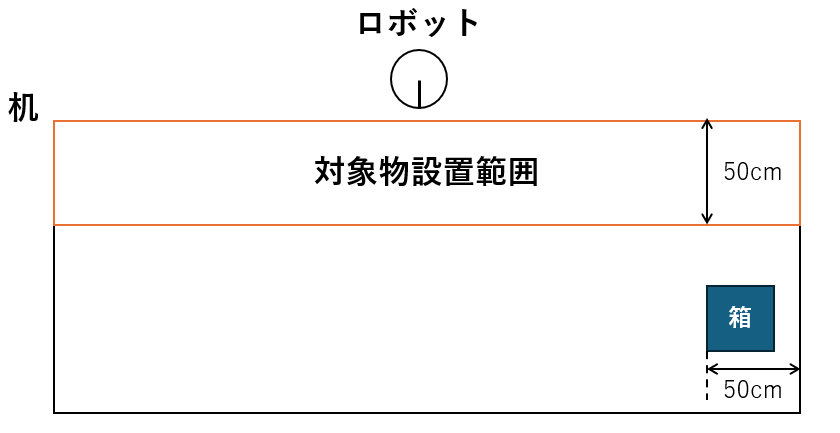
\includegraphics[width=10cm]{images/range.png}
  \caption{対象物と箱の設置範囲}
  \label{fig:range}
\end{figure}
\begin{figure}[h]
  \centering
  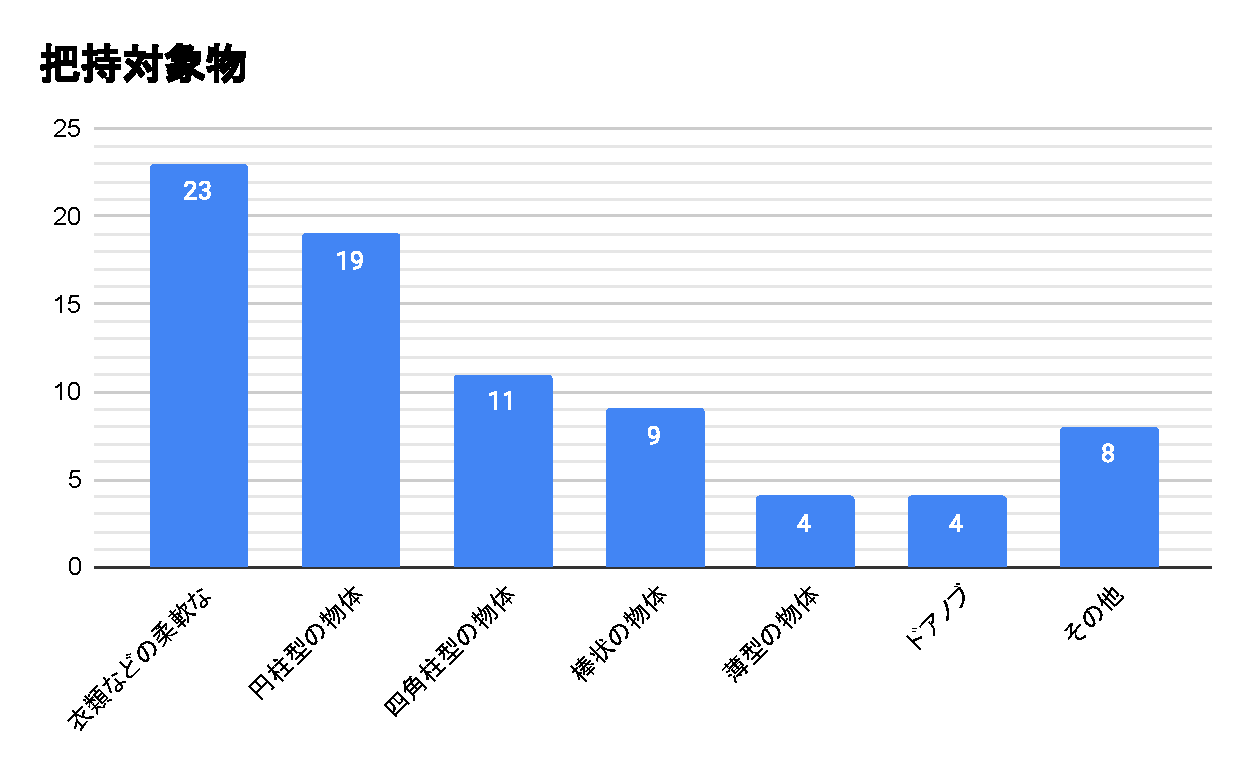
\includegraphics[width=10cm]{images/handget.pdf}
  \caption{既存のオフィスロボットが扱っている対象物}
  \label{fig:handget}
\end{figure}
\newpage